\documentclass[11pt]{article}
\usepackage{amsmath, amssymb, amscd, amsthm, amsfonts}
\usepackage{graphicx}
\usepackage{hyperref}
\usepackage{wrapfig}
\usepackage{subcaption}
% \usepackage{xeCJK}

\oddsidemargin 0pt
\evensidemargin 0pt
\marginparwidth 40pt
\marginparsep 10pt
\topmargin -20pt
\headsep 10pt
\textheight 8.7in
\textwidth 6.65in
\linespread{1.2}

\title{Failure Tolerance of Complex Networks}
\author{Yifeng Chen \\
21821113}
\date{\today}

\newtheorem{theorem}{Theorem}
\newtheorem{lemma}[theorem]{Lemma}
\newtheorem{conjecture}[theorem]{Conjecture}

\newcommand{\rr}{\mathbb{R}}
\newcommand{\al}{\alpha}
\makeatletter
\@addtoreset{equation}{section}
\makeatother
\renewcommand\theequation{\oldstylenums{\thesection}%
                   .\oldstylenums{\arabic{equation}}}
\newcommand{\expbracket}[1]{\left \langle #1  \right \rangle}

\DeclareMathOperator{\conv}{conv}
\DeclareMathOperator{\aff}{aff}

\begin{document}

\maketitle

% \begin{abstract}
% This survey presents an overview of the advances around Tverberg's theorem, focusing on the last two decades.  We discuss the topological, linear-algebraic, and combinatorial aspects of Tverberg's theorem and its applications.  The survey contains several open problems and conjectures.
% \end{abstract}
\section{Introduction}
A complex network is broadly defined as a collection of interconnected and interacting systems \cite{albert2002statistical}, where the individual subsystems (or participating agents) themselves could be complex dynamical systems. The study of complex networks is a young and active area of scientific research (since 2000) inspired largely by the empirical study of real-world networks such as computer networks, technological networks, brain networks and social networks\cite{lu2013theory}. 
Since complex networks exist broadly in our real life, the study of robustness of complex networks gains more and more attention. Early works focused on the single, isolated networks without interaction with other networks\cite{albert2000error, schneider2011mitigation}. Afterwards, effect of coupled networks are considered and analyzed using percolation theory\cite{buldyrev2010catastrophic}. In this report, we analyze the failure tolerance of both single networks and coupled networks, and carry out a simulation to verify our conclusion.

\section{Preliminaries}
% \begin{center}
% \begin{tabular}{ |c|c| } 
%  \hline
% Order Parameter & xxx  \\
%  \hline
% Critical Exponent & xxx  \\
%  \hline
% First-Order Transition & xxx  \\
%  \hline
% Second-Order Transition & xxx  \\
%  \hline
% \end{tabular}
% \end{center}
% \subsection{Phase Transition}
\begin{wrapfigure}{r}{0.5\textwidth}
  \vspace{-20pt}
  \begin{center}
    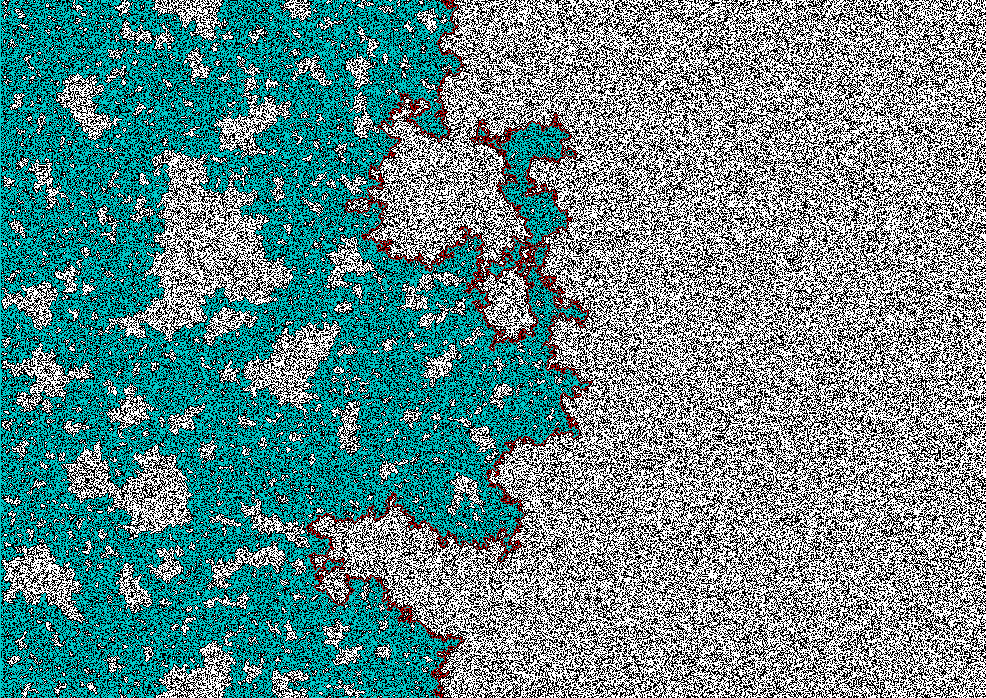
\includegraphics[width=0.45\textwidth]{Front_de_percolation.png}
  \end{center}
  \label{fig:phase_transition}
  \vspace{-20pt}
  \caption{Percolation front on a square lattice at the percolation threshold (59.3\%)}
  %\vspace{-20pt}
\end{wrapfigure}

\subsection{Percolation Theory}
% 一个复杂网络可以由一个由节点(Nodes)和边缘(Edges)组成的图(Graph)来表示. 用$p$来表示一个节点存在的概率. 我们可以提问, 当$p$给定时, 存在一个贯穿整个图的路径的可能性是多少呢? 或者,等价地,当$1-p$的节点从一个连通图中被移除时,图的连通性何时会被破坏呢? 这一问题,即站点渗透(site perlocation)问题, 可以使用平均场理论(Mean Field)来解决.
A complex network can be viewed as a graph where nodes are sites and edges are connections between them. A site is "occupied" with probability $\mathbf{p}$ or "empty" (in which case its edges are removed) with probability $1-p$. For a given $p$, what is the probability that a path exists between top and bottom? Equivalently, one can ask, given a connected graph at what fraction $1-p$ of failures the graph will become disconnected. This problem, known as site percolation, can be solved using Mean Field theory.

The Mean Field theory is applied to study phase transitions, which involves identification of a global parameter, called the \textbf{\textit{order parameter}}. It essentially quantifies the presence of order in the underlying system, which is zero (or negligible) in the disordered phase and takes on non-zero values in the ordered phase. 
In this case, order parameter, noted as $p_\infty$, is the probability that there exists a path from the top to the bottom of the network. A phase transition is caused by a continuous or a discontinuous change of the order parameter from zero to a non-zero value when an intensive system parameter (e.g., site occupation parameter) is varied across the \textbf{\textit{critical point}}.

The nature of phase transition is often broadly classified into two types (i) \textbf{first-order} phase transition - when the order parameter changes discontinuously with the intensive parameter at the critical point and, (ii)\textbf{second-order} phase transition - when the order parameter varies continuously with the intensive parameter during the phase transition. A phase transition is marked by the presence of analytical singularities or discontinuities in the functions describing macroscopic physical parameters of the system. In the vicinity of the critical point marking the phase transition, the functional form of the order parameter is often modeled using a power law with a critical exponent as stated in Eqn. \ref{eqa:criexp} below.

\begin{equation}
    p_\infty \sim (p_c-p)^{\beta},
    \label{eqa:criexp}
\end{equation}
where $p_c$ is the critical point in this system.

\subsection{Erd\"{o}s-R\'{e}nyi Network}
The Erd\"{o}s-R\'{e}nyi(ER) network is a random graph obtained by randomly distributing M links between N nodes, being a statistical ensemble with equal probability for any generated configuration. For the ER network, since links are distributed in an uncorrelated way, the degree distribution is Poissonian, i.e., the frequency of nodes with k links is
\begin{equation}
    P(k) = exp(-\lambda) \frac{\lambda^k}{k!}
    \label{eqn:erpk}
\end{equation}
A typical ER network is shown in Fig. \ref{fig:er}.

\subsection{Barab\'{a}si-Albert Network}
The Barab\'{a}si-Albert network is a network which was grown under the preferential attachment rule, i.e., at each iteration a new node is added to the network and connected to m already existing nodes with a probability of linking to a certain node proportional to the actual degree (number of links) of that node. BA network belongs to scale-free networks,  whose degree distribution follows a power law.
\begin{equation}
    P(k) = \left\{
                \begin{array}{ll}
                  ck^{-\gamma} \quad m \le k \le K\\
                  0 \quad otherwise\\
                \end{array}
              \right. ,
  \label{eqn:bapk}
\end{equation}
where $\gamma$ is the degree exponent and $K$ an upper limit due to the system finite size. As shown in Fig. \ref{fig:ba}, the power-law degree distribution favors the existence of highly connected nodes when compared with the Poisson distribution.

\begin{figure}
    \centering
    \begin{subfigure}[b]{0.3\textwidth}
        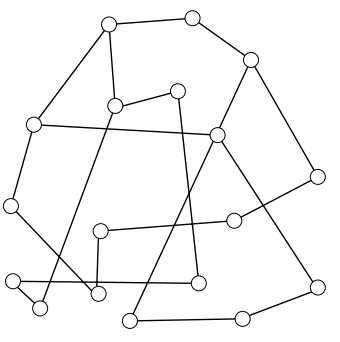
\includegraphics[width=\textwidth]{ER.png}
        \caption{A typical ER network}
        \label{fig:er}
    \end{subfigure}
    \qquad
    \begin{subfigure}[b]{0.3\textwidth}
        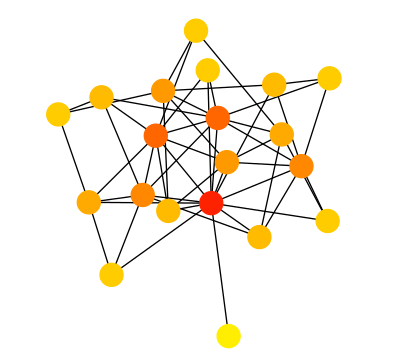
\includegraphics[width=\textwidth]{Barabasi_albert_graph.png}
        \caption{A typical BA network}
        \label{fig:ba}
    \end{subfigure}
    \caption{Two types of single networks}\label{fig:networks}
\end{figure}

\section{Single Network Robustness}
\label{single_network_robustness}
\subsection{Molloy-Reed criterion}
For a giant component to exist each node that belongs to it must be connected to at least two other nodes on average. Therefore, the average degree $k_i$ of a randomly chosen node $i$ that is part of the giant component should be at least 2. Denote with $P(k_i | i \leftrightarrow j)$ the joint probability that a node in a network with degree $k_i$ is connected to a node j that is part of the
giant component. This conditional probability allows us to determine the expected degree of node $i$ as
\begin{equation}
    \expbracket{k_i | i \leftrightarrow j} = \sum_{k_i} k_iP(k_i | i \leftrightarrow j)
    \label{eqn:degreeexp}
\end{equation}
We can write the probability use Bayes' theorem in the last term.
\begin{equation}
    P(k_i | i \leftrightarrow j) = \frac{P(k_i, i \leftrightarrow j)}{P(i \leftrightarrow j)} = \frac{P(i \leftrightarrow j | k_i)p(k_i)}{P(i \leftrightarrow j)}
\end{equation} 
For a network with degree distribution $p_k$, in the absence of degree correlations, we can write
\begin{equation}
    P(i \leftrightarrow j | k_i) = \frac{k_i}{N-1},
    \label{eqn:pijcond}
\end{equation}
which expresses the fact that we can choose between $N-1$ nodes to link to, each with probability $1/(N-1)$ and that we can try this $k_i$ times. 

\begin{equation}
    P(i \leftrightarrow j) = \frac{L}{N(N-1)/2} = \frac{\expbracket{k}N/2}{N(N-1)/2} = \frac{\expbracket{k}}{N-1} ,
    \label{eqn:pij}
\end{equation}
where L is the number of total links in the network. We can replace Eqn. \ref{eqn:pijcond}, Eqn. \ref{eqn:pij} into Eqn. \ref{eqn:degreeexp} and get
\begin{equation}
    \sum_{k_i} k_iP(k_i | i \leftrightarrow j) = \sum_{k_i} k_i \frac{k_i p(k_i)}{\expbracket{k}} = \frac{\sum_{k_i}{k_i}^2 p(k_i)}{\expbracket{k}} = \frac{\expbracket{k^2}}{\expbracket{k}}
\end{equation}
With that we arrive at the \textbf{Molloy-Reed criterion}, providing the condition to have a giant component as 
\begin{equation}
    \kappa = \frac{\expbracket{k^2}}{\expbracket{k}} > 2
\end{equation}
Networks with $\kappa < 2$ lack a giant component, being fragmented into many disconnected components. The Molloy-Reed criterion links the network’s integrity, as expressed by the presence or the absence of a giant component, to $\expbracket{k}$ and$\expbracket{k^2}$. It is valid for any degree distribution $p_k$.
 
\subsection{Critical Threshold}
The random removal of an $f$ fraction of nodes has two consequences:
\begin{itemize}
    \item It alters the degree of some nodes, as nodes that were previously connected to the removed nodes will lose some links $[k \rightarrow k^{\prime} \le k]$.
    \item It changes the degree distribution, as the neighbors of the missing nodes will have an altered degree $[p_k \rightarrow  p^{\prime}_k]$.
\end{itemize}
After we randomly remove an $f$ fraction of nodes, a node with degree $k$ becomes a node with degree $k^\prime$ with probability 
\begin{equation}
    	P(k \rightarrow k^\prime) = 
    	\left(\begin{array}{ll} 
    	    k \\
    	    k^\prime
    	\end{array} \right) f^{k - k^\prime} (1-f)^{k^\prime} \qquad k^\prime \le k
\end{equation}
Suppose the degree distribution in the original network is $p_k$, i.e. there is $p_k$ probability to have a node of degree k, the probability that we have a new node with degree $k^\prime$ in the new network is 
\begin{equation}
    p^\prime_{k^\prime} = \sum_{k=k^\prime}^{\infty} p_k P(k \rightarrow k^\prime)
\end{equation}
With $p^\prime_{k^\prime}$ defined, we can write the expectation of degree in the new network,
\begin{equation}
    \begin{split}
        \expbracket{k^\prime}_f  = & \sum_{k^\prime=0}^{\infty} k^\prime p^\prime_{k^\prime} \\
        = & \sum_{k^\prime=0}^{\infty} \sum_{k=k^\prime}^{\infty} p_k \frac{k(k-1)!}{(k^\prime-1)!(k-k^\prime)!}f^{k-k^\prime}(1-f)^{k^\prime-1}(1-f)
    \end{split}
\end{equation}
Note that we can change the sum order from $\sum_{k^\prime=0}^{\infty} \sum_{k=k^\prime}^{\infty}$ to $\sum_{k=0}^{\infty}  \sum_{k^\prime=0}^{k}$ , and get
\begin{equation}
    \begin{split}
        \expbracket{k^\prime}_f  = & \sum_{k=0}^{\infty}  \sum_{k^\prime=0}^{k} p_k \frac{k(k-1)!}{(k^\prime-1)!(k-k^\prime)!}f^{k-k^\prime}(1-f)^{k^\prime-1}(1-f) \\
         = & \sum_{k=0}^{\infty} (1-f) k p_k \sum_{k^\prime=0}^{k} \frac{(k-1)!}{(k-k^\prime)!(k^\prime-1)!}f^{k-k^\prime}(1-f)^{k^\prime-1}  \\
         = & \sum_{k=0}^{\infty} (1-f) k p_k \sum_{k^\prime=0}^{k} P(k-1 \rightarrow k^\prime -1) \\
         = & \sum_{k=0}^{\infty} (1-f) k p_k \\
         = & (1-f) \expbracket{k}
    \end{split}
\end{equation}
Similarly, we can get 
\begin{equation}
    \expbracket{{k^{\prime}}^2}_f = (1-f)^2 \expbracket{k^2} + f(1-f)\expbracket{k}
\end{equation}
To ensure the integrity of the new network, its Molloy-Reed criterion $\kappa^{\prime}=\frac{\expbracket{{k^{\prime}}^2}_f} {{\expbracket{k^\prime}}_f}$ should be above 2, thus we can get the critical threshold
\begin{equation}
    f_c = 1 - \frac{1}{\frac{\expbracket{k^2}}{\expbracket{k}}-1}
\end{equation}
No matter what degree distribution $p_k$ is, as long as more than $f_c$ nodes are \textbf{randomly} removed, the network will break down. The critical threshold $f_c$ depends only on $\expbracket{k}$ and $\expbracket{k^2}$, quantities that are uniquely determined by the degree distribution $p_k$. 

\subsection{Case Study}
\subsubsection{Erd\"{o}s-R\'{e}nyi Network}
ER network's degree observes to Poisson distribution as defined in Eqn. \ref{eqn:erpk}, hence we get 
\begin{equation}
\begin{split}
        \expbracket{k} = & \sum_{k=0}^{\infty} k e^{-\lambda} \frac{\lambda^k}{k!} \\
        = & \lambda e^{-\lambda} \sum_{k=0}^{\infty} \frac{\lambda^{k}}{k!}
\end{split}
\end{equation}
Notice that $ \sum_{k=0}^{\infty} \frac{\lambda^{k}}{k!}$ is the taylor series expansion of $e^\lambda$, leads to 	
\begin{equation}
    \expbracket{k} = \lambda e^{-\lambda} e^\lambda = \lambda
\end{equation}
Similarly, we can solve $\expbracket{k^2}$
\begin{equation}
\begin{split}
    \expbracket{k^2} = & \sum_{k=0}^{\infty} k^2 e^{-\lambda} \frac{\lambda^k}{k!} \\
    = & \lambda^2 - \lambda
\end{split}
\end{equation}
Then the critical threshold for an ER network is 
\begin{equation}
    f_c = 1 - \frac{1}{\lambda}
    \label{eqn:fcer}
\end{equation}
Hence, the denser is a random network, the higher is its $f_c$, i.e. the more nodes we need to remove to break it apart. Furthermore Eqn. \ref{eqn:fcer} predicts that $f_c$ is always finite, hence a random network must break apart after the removal of a finite fraction of nodes.


\subsubsection{BA Network(scale-free)}
BA network's degree observes to heavy-tail distribution as defined in Eqn. \ref{eqn:bapk}, hence we get 
\begin{equation}
    \expbracket{k} = \sum_{k=m}^\infty ck^{1-\gamma} = \frac{c}{2-\gamma} x^{2-\gamma} \bigg|_{x=m}^{x=\infty}  
\end{equation}
\begin{equation}
    \expbracket{k^2} = \sum_{k=m}^\infty ck^{2-\gamma} = \frac{c}{3-\gamma} x^{3-\gamma} \bigg|_{x=m}^{x=\infty}  
\end{equation}
Then we have 
\begin{equation}
    f_c = 
    \left\{
    \begin{array}{cc} 
         & 1 \qquad 0<\gamma<3 \\
         & 1 - \frac{1}{\frac{\gamma-2}{\gamma-3}m-1}  \qquad \gamma>3
    \end{array} \right.
\end{equation}
For $\gamma > 3$ the critical threshold $f_c$ depends only on $\gamma$ and $m$, hence $f_c$ is independent of the network size $N$. In this regime a scale-free network behaves like a random network: it falls apart once a finite fraction of its nodes are removed.
For $\gamma < 3$, in order to fragment an infinite scale-free network we must remove all of its nodes. Scale-free networks can withstand an arbitrary level of random failures without breaking apart. The hubs are responsible for this remarkable robustness. Indeed, random node failures by definition are blind to degree, affecting with the same probability a small or a large degree node. Yet, in a scale-free network we have far more small degree nodes than hubs. Therefore, random node removal will predominantly remove one of the numerous small nodes as the chances of selecting randomly one of the few large hubs is negligible. These small nodes contribute little to a network’s integrity, hence their removal does little damage.

%Therefore random networks have a finite threshold, but for scale-free networks with $\gamma < 3$ the breakdown threshold converges to one. In other words, we need to remove all nodes to break a scale-free network apart, indicating that these networks show an extreme robustness to random failures. The origin of this extreme robustness is the large $\expbracket{k^2}$ term. Given that for most real networks $\expbracket{k^2}$ is larger than the random expectation, enhanced robustness is a generic property of many networks. This robustness is rooted in the fact that random failures affect mainly the numerous small nodes, which play only a limited role in maintaining a network’s integrity.

\section{Coupled Network Robustness}
Let's consider two networks, namely A and B. When a node $A_i$ in A is removed, its connected nodes in A and B are removed as well. The same procedure takes place recurrently and can cause a cascaded failure between these two networks. In Sec. \ref{single_network_robustness}, we show that in single networks, when a fraction of nodes $f$ is removed, a percolation transition occurs at a certain threshold $f_c$. Below this threshold, a giant mutually connected connected cluster exists, otherwise, the entire system turns completely fragmented.
\subsection{Coupled Erd\"{o}s-R\'{e}nyi Network}
For two coupled ER networks, the problem can be solved using generating functions~\cite{shao2008fractal}. When the two networks have the same degree, $\expbracket{k}_A = \expbracket{k}_B = \lambda$, the value of $f_c$ is 
\begin{equation}
    f_c = 1 - \frac{1}{2 \lambda z(1-z)}, 
\end{equation}
where $z \approx 0.28467 $ is the solution of equation $z = exp((z-1) / 2z)$. Approximately, we have \begin{equation}
    f_c = 1 - \frac{2.4554}{\lambda}
\end{equation}
Compared to Eqn. \ref{eqn:fcer}, this reveals that coupled ER networks are more vulnerable than stand-alone ER networks. As the ratio between the average degrees of two networks decreases, the threshold $f_c$ increases, i.e., the coupled network becomes more resilient to failures. In the limit where this ratio becomes zero, the single-network feature is recovered, obviously. 

\subsection{Scale-free Networks}
 Analogously to ER networks, the coupling between scale-free networks significantly increases the vulnerability of the system, with a lower $f_c$ compared to the case of a single network. Since hubs can have a low-degree counterpart node, their vulnerability evinces with the coupling. In contrast to single networks, the broader the degree distribution the lower is $f_c$, i.e., the smaller the fraction of nodes that needs to be removed to fully fragment the system.
 
 \section{Simulations}
 In single networks, we both visualize the case of ER network and scale-free network. We use $P_\infty$ , the probability of one node belonging to the largest connected center, to measure the connectivity of networks. As plotted below, a second-order phase transition take place in both types of networks when more nodes are being removed. We use Configure Model to generate a scale-free network of arbitrary $\gamma$. Specifically, it first generates a random degree sequence and wires nodes together afterwards.

 \begin{figure}
    \centering
    \begin{subfigure}[b]{0.45\textwidth}
        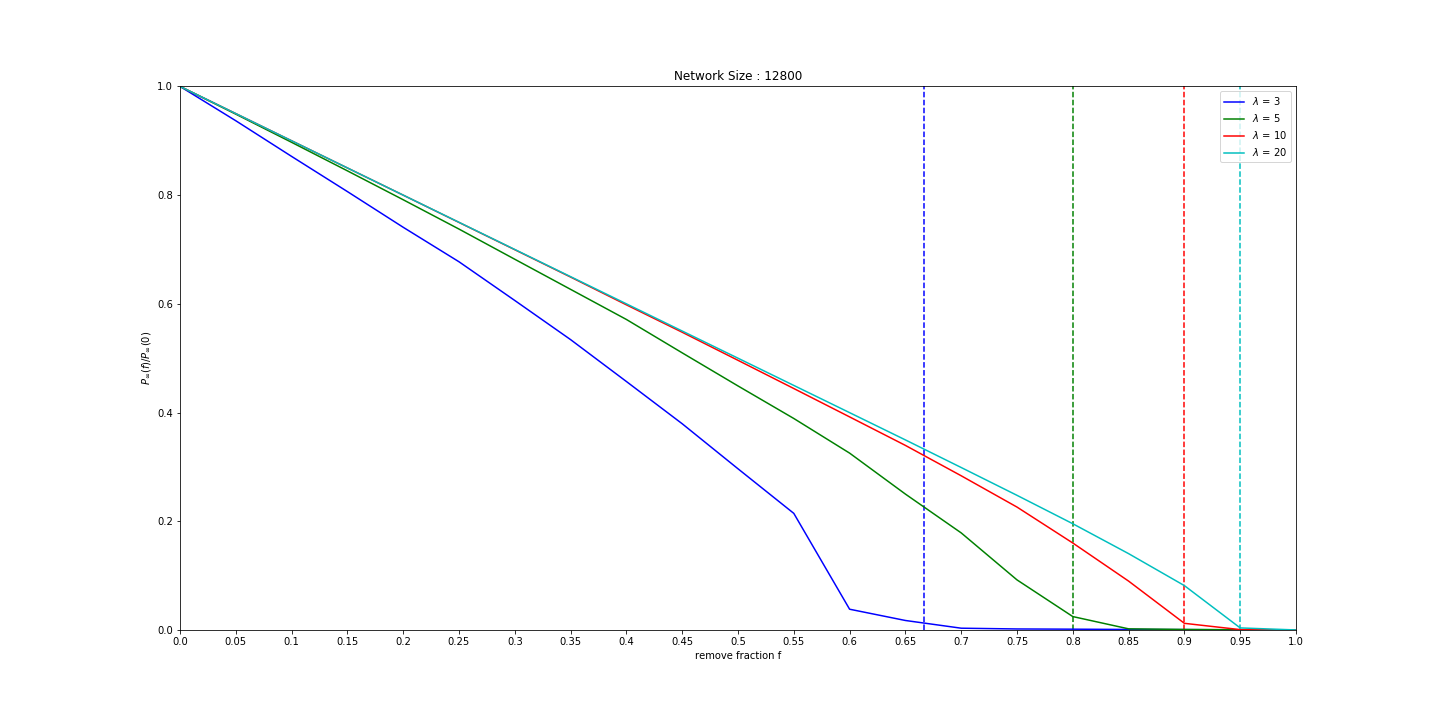
\includegraphics[width=\textwidth]{ser.png}
        \caption{ER network}
        \label{fig:er}
    \end{subfigure}
    \quad
    \begin{subfigure}[b]{0.45\textwidth}
        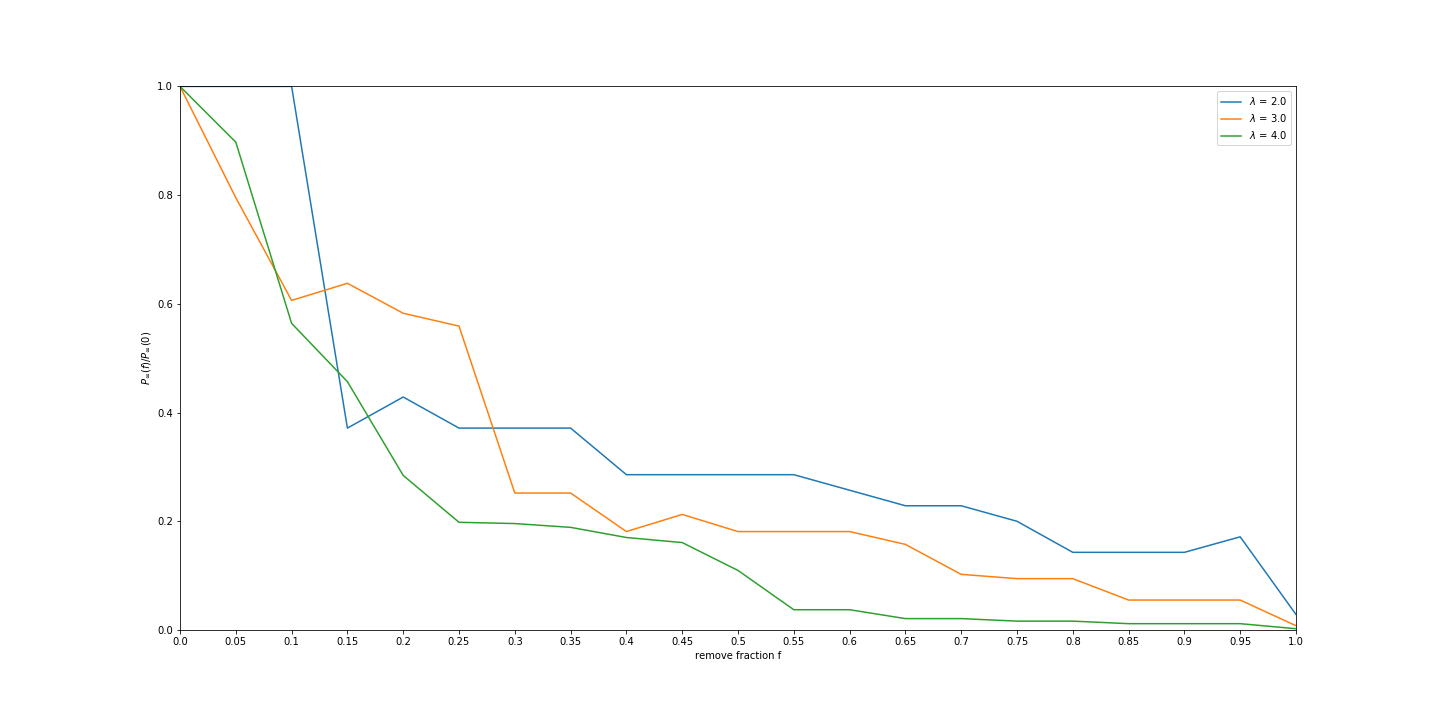
\includegraphics[width=\textwidth]{sba.png}
        \caption{Scale-free network}
        \label{fig:ba}
    \end{subfigure}
    \caption{Single Network Simulation}\label{fig:networks}
\end{figure}
 
 
\newpage
\bibliographystyle{alpha}
\bibliography{references} % see references.bib for bibliography management

\end{document}
